% !TeX program = xelatex
% ↑ Automatische Auswahl für XeLaTeX compiler

% Das ist mein Template für die TX000 Arbeiten. Nicht perfekt, also falls ihr Verbesserungsvorschläge habt, stellt gerne einen Pull-Request. https://github.com/NikomitK/TX000_Template
% Bitte lasst auch einen star auf github da, danke.
% Wenn ihr die cite funktion von LaTeX nutzen wollt, müsst ihr einfach die Quellen im bibtex Format in die sources.bib datei kopieren, google scholar z.B. hat bei den Quellen einen Button mit dem man das so bekommt, auch viele andere websites.
% Bilder kommen in den images Ordner, den müsst ihr beim abrufen eines Bildes nicht angeben, passiert automatisch.


% Trag hier deine Daten ein, die entsprechenden Felder werden automatisch angepasst.
\def\meinTitel{Skalierbare Chatapplikation mit LLM-Moderation}
\def\artDerArbeit{Verteilte Systeme Ausarbeitung}
\def\meinName{Nikolas Bodenmüller,\\Fabian Sigmund}
\def\meinKurs{TINF22F}
\def\meineMatrikelNr{2399231, 7982497}
\def\abgabeDatum{16.12.2024}
%-----------------------------------------------------------------------------------


\documentclass[12pt]{report}
\usepackage[heightrounded]{geometry}
\geometry{
	a4paper,
	lmargin=3.1cm, %Seitenrand left
	tmargin=2.8cm, %Seitenrad top
	headsep=35pt %Abstand von Kopfzeile
}
\usepackage[onehalfspacing]{setspace}
\usepackage[compact]{titlesec}
\usepackage{cite} % Zitierungen
\usepackage{struktex} % Struktogramme
\usepackage{array} % kp hat chatgpt benutzt
\usepackage{longtable} % Tabelle über einen seitenumbruch
\usepackage[nohyperlinks, printonlyused]{acronym} % abkürzungsverzeichnis
\usepackage{blindtext} % LoremIpsum
\usepackage{fancyhdr} % Kopf- und Fußzeile
\usepackage[export]{adjustbox} % Bilder alignment
\usepackage{stfloats} % Tabular at bottom
%\usepackage[table]{xcolor} %Tabellen farben
\usepackage{tabularx} % Anpassbarere tabellen

\usepackage[utf8]{inputenc} % this is needed for umlauts
\usepackage[ngerman]{babel} % this is needed for umlauts
\usepackage[T1]{fontenc}    % this is needed for correct output of umlauts in pdf


\usepackage{subcaption} % Für subfigures glaub


\usepackage{tikz} % Zum zeichnen
\usetikzlibrary{calc}
\usetikzlibrary{shapes.geometric, arrows}

%--------------------Flowcharts--------------------
\tikzstyle{startstop} = [rectangle, rounded corners, minimum width=3cm, minimum height=1cm,text centered, draw=black, fill=red!30]
\tikzstyle{io} = [trapezium, trapezium left angle=70, trapezium right angle=110, minimum width=3cm, minimum height=1cm, text centered, draw=black, fill=blue!30]
\tikzstyle{process} = [rectangle, minimum width=3cm, minimum height=1cm, text centered, draw=black, fill=orange!30]
\tikzstyle{decision} = [diamond, minimum width=3cm, minimum height=1cm, text centered, draw=black, fill=green!30]
\tikzstyle{arrow} = [thick,->,>=stealth]
%--------------------------------------------------


%--------------------Codeblöcke--------------------
\usepackage{listings} %Für Codeblöcke
\usepackage{color} %Farben für Codeblöcke?
\definecolor{dkgreen}{rgb}{0,0.6,0}
\definecolor{gray}{rgb}{0.5,0.5,0.5}
\definecolor{mauve}{rgb}{0.58,0,0.82}

\lstset{
	language=Java,
	aboveskip=3mm,
	belowskip=3mm,
	showstringspaces=false,
	columns=flexible,
	basicstyle={\small\ttfamily},
	numbers=none,
	numberstyle=\tiny\color{gray},
	keywordstyle=\color{blue},
	commentstyle=\color{dkgreen},
	stringstyle=\color{mauve},
	breaklines=true,
	breakatwhitespace=true,
	tabsize=3
}

\lstset{
	language=Python,
	basicstyle=\ttfamily\small,
	keywordstyle=\color{blue},
	stringstyle=\color{red},
	commentstyle=\color{gray},
	backgroundcolor=\color{gray!10},
	showstringspaces=false,
	numbers=left,
	numberstyle=\tiny\color{gray},
	numbersep=5pt
}
%-------------------------------------------------

\usepackage{graphicx} %Package für Bilder
\graphicspath{ {./images/} } %Ordner für Bilder

\sloppy % damit lange Wörter nicht über die Zeile hinausgeschrieben werden.

%--------------------Chapter Heading--------------------
\makeatletter
\def\@makechapterhead#1{%
	\vspace*{-20\p@}%
	{\parindent \z@ \raggedright \normalfont
		\ifnum \c@secnumdepth >\m@ne
		%\huge\bfseries \@chapapp\space \thechapter
		\Huge\bfseries \thechapter.\space%
		%\par\nobreak
		%\vskip 20\p@
		\fi
		\interlinepenalty\@M
		\Huge \bfseries #1\par\nobreak
		\vskip 20\p@
}}
\makeatother
\makeatletter
\def\@makeschapterhead#1{%
	\vspace*{-20\p@}%
	{\parindent \z@ \raggedright \normalfont
		%\huge\bfseries \@chapapp\space \thechapter
		\Huge\bfseries\space%
		%\par\nobreak
		%\vskip 20\p@
		\interlinepenalty\@M
		\Huge \bfseries #1\par\nobreak
		\vskip 20\p@
}}
\makeatother
%-------------------------------------------------------

%\addto\captionsngerman{\renewcommand{\listfigurename}{}}
 % titel von abbildungsverzeichnis weg?

\setlength\parindent{0pt} %Auto Einrücken deaktivieren


%-------------Setup für Inhaltsverzeichnis--------------
\renewcommand{\contentsname}{Inhaltsverzeichnis} %Umbenennung TOC

\usepackage{tocloft} % Formatierung TOX

\setlength{\cftbeforetoctitleskip}{0pt}

\setlength{\cftsubsecnumwidth}{4em} %abstand kapitelnummer - titel

\renewcommand{\cfttoctitlefont}{\huge\bfseries}
\renewcommand{\cftloftitlefont}{\huge\bfseries}

\renewcommand\cftchapfont{\Large\bfseries}
\renewcommand\cftchappagefont{\large}

\renewcommand\cftsecfont{\large\bfseries}
\renewcommand\cftsecpagefont{\large}

\renewcommand\cftsubsecfont{\large}
\renewcommand\cftsubsecpagefont{\large}

\renewcommand\cftsubsubsecfont{\normalsize}
\renewcommand\cftsubsubsecpagefont{\normalsize}


\renewcommand\cftchapafterpnum{\par\addvspace{8pt}}
\renewcommand\cftsecafterpnum{\par\addvspace{8pt}}
\renewcommand\cftsubsecafterpnum{\par\addvspace{6pt}}
\renewcommand\cftsubsubsecafterpnum{\par\addvspace{6pt}}
%-------------------------------------------------------


%------------------Setup für LoF/LoT--------------------
\makeatletter
\renewcommand{\@cftmakeloftitle}{}
\renewcommand{\@cftmakelottitle}{}
\makeatother
\setlength{\cftfigindent}{0em} % change indentation of e.g. "Figure 1" within list of figures
\renewcommand\cftfigfont{\large}
\renewcommand\cftfigpagefont{\large}
\setlength{\cfttabindent}{0em} % change indentation of e.g. "Figure 1" within list of figures
\renewcommand\cfttabfont{\large}
\renewcommand\cfttabpagefont{\large}
\setlength{\cftbeforeloftitleskip}{0pt}
\setlength{\cftbeforelottitleskip}{0pt}
%-------------------------------------------------------


%----------------Setup für Verlinkungen-----------------
\usepackage{hyperref}
\hypersetup{
	colorlinks,
	citecolor=black,
	filecolor=black,
	linkcolor=black,
	urlcolor=black
}
%-------------------------------------------------------


%-------------Kopf-/Fußzeile für Titlepage--------------
\fancypagestyle{titlepage}
{
	\fancyhead[L]{
\includegraphics[scale=0.09]{firmenlogo}}
	\fancyhead[R]{
\includegraphics[scale=0.25]{dhbw}}
	\renewcommand{\headrulewidth}{0pt}
	\fancyfoot[C]{}
}
%-------------------------------------------------------

\begin{document} 
	
	\begin{titlepage}
		\thispagestyle{titlepage}
		\newcommand\HRule{\rule{\textwidth}{1pt}} %Titellinien

		
		\begin{center}
			
			\vspace*{2cm}
			
			%Title
			\begin{spacing}{2}
				{ \huge \bfseries \MakeUppercase{\meinTitel}}
				%{ \large \bfseries subTitle}\\[0.4cm]
			\end{spacing}
			
			\vspace*{1.5cm}
			
			%Art der Arbeit
			\Large \artDerArbeit
			
			\vspace*{3cm}
			
			%Hochschule
			{\LARGE Studiengang Informatik}\\
			{\LARGE an der Dualen Hochschule}\\
			{\LARGE Baden-Württemberg Stuttgart}\\

			\vspace*{2.5cm}
			
			\Large von Nikolas Bodenmüller und Fabian Sigmund
			
			\large Matrikelnummer: \meineMatrikelNr  
			
			\large Kurs: \meinKurs
			
			\vspace*{1.5cm}
			
			\Large Abgabedatum: \abgabeDatum
			
			
		\end{center}
		
	\end{titlepage}


%------------------Kopf- und Fußzeile-------------------
%\spacing{1.5}
\spacing{1}

\fancypagestyle{plain}{
	\fancyfoot[L]{\meinName\\
		 \meinKurs}
	\fancyfoot[C]{Seite \thepage\ }% von \pageref{LastPage}}
	\fancyfoot[R]{\abgabeDatum}
}

\pagestyle{plain}
\fancyhead{}


\fancyhead[C]{\nouppercase\leftmark}
\fancyhead[R]{
\includegraphics[scale=0.25]{dhbw}}

\renewcommand{\footrulewidth}{0.4pt} %Linie für Fußzeile


\renewcommand{\sectionmark}[1]{\markboth{#1}{}} 
%-------------------------------------------------------

\pagenumbering{Roman}
\newpage

%------------------Inhaltsverzeichnis-------------------

\addcontentsline{toc}{chapter}{\protect\numberline{}Inhaltsverzeichnis}
\tableofcontents
\addtocontents{toc}{}
\thispagestyle{plain}
%-------------------------------------------------------

%********************************
%Abbildungsverzeichnis
%********************************
\newpage
\chapter*{Abbildungsverzeichnis}
\addcontentsline{toc}{chapter}{\protect\numberline{}Abbildungsverzeichnis}

\listoffigures


%Speichern des page counters, um bei Literaturverzeichnis weiter zu zählen.
\newcounter{frontmatterPage}
\addtocounter{frontmatterPage}{\value{page}} 

\newpage
\pagenumbering{arabic}
\chapter{Einleitung}

\chapter{Architektur}
\section{Allgemein}
\subsection{Aufbau}
Für die Umsetzung des Systems wurde eine Microservice-Architektur gewählt. Die Nachrichten werden zwischen Frontend und Backend über das WebSocket-Protokoll ausgetauscht, wobei es einen Fallback auf HTTP gibt. Zwischen instanzen des Backends werden Nachrichten als Events ausgetauscht. Die Architektur wird in Abbildung \ref{fig:Architektur} dargestellt.
\begin{figure}[htbp]
	\centering
	\includegraphics[width=\linewidth]{architektur}
	\caption{Architekturdiagramm der Chatapplikation}
	\label{fig:Architektur}
\end{figure}
\subsection{Architekturelle Entscheidungen}

\section{Systemkomponenten}
\subsection{Welche Komponenten}
Die Architektur des Systems ist in sechs Komponenten aufgeteilt. 
\begin{enumerate}
	\item \textbf{Frontend}: 
	\begin{itemize}
		\item Grafische Benutzeroberfläche
		\item Speichert lokal den Chatverlauf
		\item Mehrere Instanzen hinter einem Loadbalancer
	\end{itemize}
	\item \textbf{Chat-MS}
	\begin{itemize}
		\item Akzeptiert Nachrichten vom Frontend
		\item Sendet eingehende Nachrichten an Frontend
		\item Validiert Nachrichten über Moderations-MS
		\item Mehrere Instanzen hinter einem Loadbalancer
		\item Austausch über Events
	\end{itemize}
	\item \textbf{History-MS}
	\begin{itemize}
		\item Liefert Chatverlauf ab einem spezifizierten Zeitpunkt
		\item Mehrere Instanzen hinter einem Loadbalancer
	\end{itemize}
	\item \textbf{Moderations-MS}
	\begin{itemize}
		\item Überprüft Nachrichten auf anstößigen Inhalt
		\item Mehrere Instanzen in einem Connectionpool
	\end{itemize}
	\item \textbf{Datenbank}
	\begin{itemize}
		\item Speichert Nachrichten 
		\item Speichert Nutzer
		\item Eine Instanz
	\end{itemize}
	\item \textbf{Messaging-Broker}
	\begin{itemize}
		\item Austausch von Nachrichten zwischen Chat-MS instanzen
	\end{itemize}
\end{enumerate}

\subsection{Kommunikation zwischen Komponenten}
In Abbildung \ref{fig:seq_start} wird die Kommunikation zwischen den Komponenten dargestellt, wenn ein Nutzer die Verbindung zum Frontend aufbaut.
\begin{figure}[htbp]
	\centering
	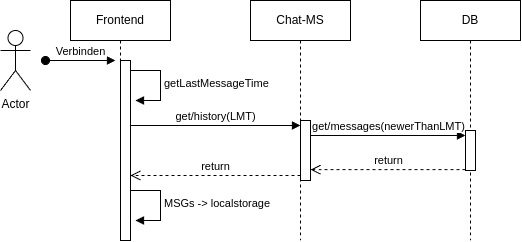
\includegraphics[width=\linewidth]{sequence_start}
	\caption{Sequenzdiagramm für eine gesendete Nachricht}
	\label{fig:seq_start}
\end{figure}

In Abbildung \ref{fig:seq_msg} wird die Kommunikation zwischen den Komponenten dargestellt, wenn ein Nutzer im Frontend eine Nachricht absendet.
\begin{figure}[htbp]
	\centering
	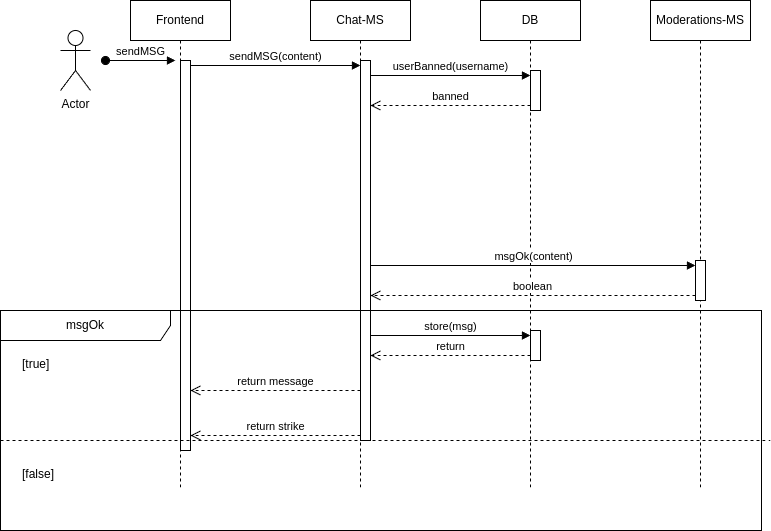
\includegraphics[width=\linewidth]{sequence_msg}
	\caption{Sequenzdiagramm für eine gesendete Nachricht}
	\label{fig:seq_msg}
\end{figure}

\section{Funktionale und nicht-funktionale Anforderungen}

\subsection{Funktionale Anforderungen}
\begin{itemize}
	\item Das System ermöglicht das Senden und Empfangen von Nachrichten zwischen Clients in Echtzeit.
	\item Die Loadbalancer sorgen für eine gleichmäßige Verteilung der Anfragen an die verfügbaren Backend-Instanzen.
	\item Eingehende Nachrichten werden vom Moderations-LLM überprüft, um unzulässige Inhalte zu filtern.
	\item Der History-MS speichert Nachrichten und Chat-Historien und stellt sie bei Bedarf zur Verfügung.
	\item Neue Instanzen von Chat-Server oder History-MS können hinzugefügt oder entfernt werden, um Lastspitzen zu bewältigen.
	\item Chat-Daten werden dauerhaft in der Datenbank gespeichert, um den Zugriff auf frühere Nachrichten sicherzustellen.
	\item Die Kommunikation zwischen Chat-Server und History-MS erfolgt asynchron über einen Nachrichten-Broker wie Kafka.
	\item Bei Ausfällen einzelner Server werden Anfragen automatisch auf andere Instanzen umgeleitet.
\end{itemize}

\subsection{Nicht-Funktionale Anforderungen}
\begin{itemize}
	\item Eine horizontale Skalierung der Services ermöglicht die Bewältigung einer steigenden Anzahl von Benutzern.
	\item Nachrichten sollen innerhalb von Millisekunden verarbeitet und zugestellt werden.
	\item Das System bleibt fehlertolerant, sodass Ausfälle einzelner Komponenten keine Auswirkungen auf das Gesamtsystem haben.
	\item Die Nachrichtenübertragung bleibt zuverlässig, sodass keine Nachrichten verloren gehen.
	\item Der modulare Aufbau des Codes und der Infrastruktur erleichtert zukünftige Änderungen und Erweiterungen.
\end{itemize}


\chapter{Umsetzung}

In diesem Kapitel wird die praktische Realisierung der zuvor beschriebenen Systemarchitektur vorgestellt. Dabei wird zunächst die konkrete Implementierung der einzelnen Komponenten erläutert und auf die wichtigsten technischen Entscheidungen eingegangen. Anschließend werden mögliche Alternativen und Schwierigkeiten bei der Umsetzung zur aktuellen Umsetzung diskutiert, um weitere Lösungsansätze aufzuzeigen und das Projekt kritisch zu reflektieren.

\section{Implementierung}

\subsection{Chat-Server}
Der Chat-Server wurde in Java unter Verwendung des Spring Boot Frameworks entwickelt. Im folgenden sollen die Hauptfunktionalitäten des Chat-Servers erläutert werden.\newline

Eingehende Nachrichten von WebSocket-Clients werden vom Server empfangen und an den \texttt{ChatService} weitergeleitet. Dort erfolgt eine Validierung und Verarbeitung der Nachrichten, bevor sie an die entsprechenden Empfänger verteilt werden. Bei identifizierten unangemessenen Inhalten wird automatisch eine Systemnachricht generiert, und der betreffende Benutzer wird sanktioniert. Für die asynchrone Nachrichtenübermittlung kommt Apache Kafka zum Einsatz, um die Nachrichten zwischen den Backend Replika zu verteilen.\newline

Validierte Nachrichten werden in einer Elasticsearch-Datenbank gespeichert, um einen dauerhaften Nachrichtenverlauf zu gewährleisten. Die Benutzerverwaltung erfolgt ebenfalls in dieser Datenbank, wobei Informationen wie Benutzerstrikes und Sperren automatisch aktualisiert werden.\newline

Für die Validierung der Nachrichten nutzt der \texttt{LLMService} Verbindungen aus dem \texttt{LLMConnectionPool}. Der \texttt{LLMConnectionPool} verwaltet die verfügbaren API-Verbindungen mithilfe einer Round-Robin-Logik, unterstützt durch Redis als Zählmechanismus. Durch die Verwendung der \texttt{WebClient}-Klasse werden HTTP-Verbindungen effizient wiederverwendet, was die Leistung und Ressourcennutzung optimiert \cite{spring-webclient}. Sollte ein API-Aufruf fehlschlagen, wird die Anfrage durch das \texttt{RetryTemplate} automatisch wiederholt. Dies stellt sicher, dass bei einem Ausfall eines LLM-Containers die Anfrage an einen anderen Container weitergeleitet wird, wodurch die Ausfallsicherheit und Zuverlässigkeit des Systems erhöht wird.\newline

\subsection{LLM-Service}

Der LLM-Service wurde in Python umgesetzt. Die Wahl fiel auf Python, da die Sprache eine breite Auswahl an Machine Learning Bibliotheken bietet. Für den LLM-Service wurde die \texttt{transformers} Bibliothek verwendet, da diese vortrainierte Modelle bereitstellt, die durch wenige Zeilen Code eingebunden werden können. Jedoch konnten wir kein Modell finden, das sowohl Deutsche Texte als auch Englische Texte klassifizieren kann.
\newline\newline
Insgesamt wurden deshalb zwei Modelle für die Lösung genutzt:

\begin{center}
	\texttt{ml6team/distilbert-base-german-cased-toxic-comments} (Deutsches Modell) \texttt{unitary/multilingual-toxic-xlm-roberta} (Multilinguales Modell)
\end{center}

Das deutsche Modell basiert auf dem \texttt{distilbert/distilbert-base-german-cased} und wurde speziell auf toxische Kommentare trainiert. Unsere Wahl wurde durch ein Konferenzpaper inspiriert, das dieses Modell zur Analyse von Verschwörungstheorien in Telegram-Gruppen erfolgreich einsetzte \cite{weigand-etal-2022-conspiracy}. Ergänzend hierzu wurde ein mehrsprachiges Modell eingesetzt, um toxische Inhalte in verschiedenen Sprachen zuverlässig zu klassifizieren. Die Entscheidung fiel auf das \texttt{unitary}-Modell, das auf \texttt{XLM-RoBERTa} basiert und durch einen hohen F1-Score überzeugt, was Fehlklassifikationen deutscher Nachrichten als toxisch minimiert \cite{model-comparison}.\newline

Das \texttt{unitary}-Modell kann unter anderem Englisch, Italienisch und Russisch klassifizieren, jedoch nicht Deutsch. Um diese Einschränkung auszugleichen und Fehlklassifikationen zu vermeiden, setzen wir gezielt auf zwei spezialisierte Modelle - ein Ansatz, der in der Literatur als Multi-Model-Ansatz (\textit{Multi-Model Approach}) bekannt ist. Dieses Vorgehen kombiniert die Stärken beider Modelle und sorgt für eine präzisere Erkennung toxischer Inhalte.\newline

Ein ähnlicher Multi-Model-Ansatz wurde von Tran und Kruschwitz (2021) im Rahmen des GermEval 2021 Shared Tasks verfolgt. Sie kombinierten mehrere BERT-Modelle mittels Hard Voting, um die Klassifikation toxischer Kommentare zu optimieren \cite{tran2021ensemble}. Im Gegensatz dazu verwenden wir aus Effizienz- und Performancegründen bewusst nur zwei Modelle. Da Hard Voting bei dieser geringen Modellanzahl nicht möglich ist, priorisieren wir das multilinguale Modell, sofern dessen Konfidenzwert besonders hoch ist, um eine präzise Klassifikation sicherzustellen.\newline

Die folgende Code-Implementierung zeigt die Auswahllogik für das beste Klassifikationsergebnis: Wenn das mehrsprachige Modell einen Konfidenzwert über 0,9 erreicht, wird dessen Ergebnis priorisiert. Andernfalls wird das Ergebnis des deutschen Modells verwendet. Dies reduziert die Wahrscheinlichkeit, dass deutsche Nachrichten fälschlicherweise als toxisch eingestuft werden.
\begin{figure}[h]
	\centering
	\begin{lstlisting}
		best_result = multilingual_result if multilingual_result[0]['score'] > 0.9 else german_result
	\end{lstlisting}
	\caption{Python-Code zur Auswahl des besten Klassifikationsergebnisses.}
	\label{fig:best_result_selection}
\end{figure}

\subsection{History-MS}
Der History Microservice (History-MS) ist ebenfalls im Spring Boot umgesetzt. Er ermöglicht es Benutzern, über eine REST-API auf den Nachrichtenverlauf zuzugreifen und somit auch nach einer Unterbrechung nahtlos den vorherigen Chatverlauf einzusehen. Dabei werden die Nachrichten in einer Elasticsearch-Datenbank gespeichert, die eine effiziente Speicherung und Abfrage der Daten ermöglicht. Die REST-API stellt einen Endpunkt bereit, über die Benutzer den Nachrichtenverlauf abrufen können, indem sie einen bestimmten Zeitstempel angeben, ab dem die Nachrichten angezeigt werden sollen.


\subsection{Frontend}
Das Frontend der Chat-Anwendung wurde mit Angular entwickelt und bietet den Benutzern eine einfache Oberfläche zum Senden und Empfangen von Nachrichten. Es stellt Anfragen an den zuvor genannten Chat-Server und den History-MS. Falls der aktuell verbundene Chat-Server abstürzt, verbindet sich das Frontend automatisch mit einem andern verfügbaren Replika, um die Kommunikation aufrechtzuerhalten.
\section{Mögliche Alternativen und zusätzliche Schwierigkeiten}

Während der Entwicklungsphase wurden verschiedene Alternativen in Betracht gezogen. Für den Chat-Server hätten andere Programmiersprachen verwendet werden können, jedoch entschieden wir uns für uns bereits bekannte Technologien, um die Entwicklung effizienter zu gestalten. Für den LLM-Service wurde auch die Möglichkeit in Erwägung gezogen, ein eigenes Modell zu trainieren, um maximale Kontrolle über die Textmoderation zu erhalten. Allerdings hätte das eigene Training erheblichen Zeitaufwand erfordert, weshalb wir uns für bestehende vortrainierte Modelle entschieden.\newline

Bei der Wahl der Datenbank nutzten wir zunächst MongoDB, entschieden uns jedoch später dafür, Elasticsearch auszuprobieren, um dessen spezialisierte Such- und Analysefunktionen besser zu verstehen. Im Frontend-Bereich wären ebenfalls alternative Frameworks denkbar gewesen, jedoch entschieden wir uns für eine vertraute Lösung, um die Entwicklungszeit zu minimieren.\newline

Eine wesentliche technische Herausforderung war die hohe Rechenintensität der Container für den LLM-Service. Um die Belastung zu reduzieren und die Präsentation reibungslos durchzuführen, wurde der LLM-Service auf einem separaten Laptop gehostet, während die restliche Anwendung auf einem anderen Laptop lief. Die Kommunikation zwischen den Laptops erfolgte über ein Netzwerk, was eine bessere Lastverteilung und stabile Demonstrationsbedingungen sicherstellte.\newline

\chapter{Reflexion}


%********************************
%Literaturverzeichnis
%********************************
\newpage
\pagenumbering{Roman}
\setcounter{page}{\value{frontmatterPage}} %Bei \pagenumbering wird Seitenzähler zurückgesetzt, hier wird der gespeicherte Wert vom frontmatter weitergeführt
\addtocounter{page}{1}
\addcontentsline{toc}{chapter}{\protect\numberline{}Literaturverzeichnis}

%Quellenverzeichnis
\renewcommand{\refname}{Literaturverzeichnis}
\bibliographystyle{IEEEtran}
\bibliography{./sources/bibliography}


\end{document}